
\section{Background}
\subsection{GPU Memory Architecture}
Modern GPUs employ a complex execution pipeline and memory hierarchy to support concurrent execution of parallel threads. A typical GPU
consists of multiple Streaming Multiprocessors (SMs). Each SM includes multiple Single-Instruction-Multiple-Thread (SIMT) units, each of
which has multiple lanes of execution. Threads scheduled in the same SIMT unit are called a warp, which is the smallest scheduling unit in
GPU. Like a modern CPU, a GPU consists of multiple memory hierarchies. The thread-local registers are the fastest memory component, having
the lowest access latency (1-2 cycles). The SM local L1 caches and shared memory provide a larger storage capacity over the thread-local
registers but have modestly higher accessing latency of around 30 cycles. All the SMs share a unified L2 cache that provides an accessing
latency of about 200 cycles. The off-chip global memory, similar to the RAM in a CPU system, provides the largest memory storage capacity
on the GPU but has the longest accessing latency of around 500 cycles. Local memory resides in global memory and is used to hold variables with dynamic indexing or too large to fit into registers. It has the same access latency as global memory. The key to optimizing memory performance is to make use of the fast
memory sub-systems (i.e., registers and shared memory) and reduce the number of memory accesses or transactions. Our work is designed to
provide such capabilities for convolution operations.

\subsection{Convolution Operations}
\begin{figure}[t!]
\centering
  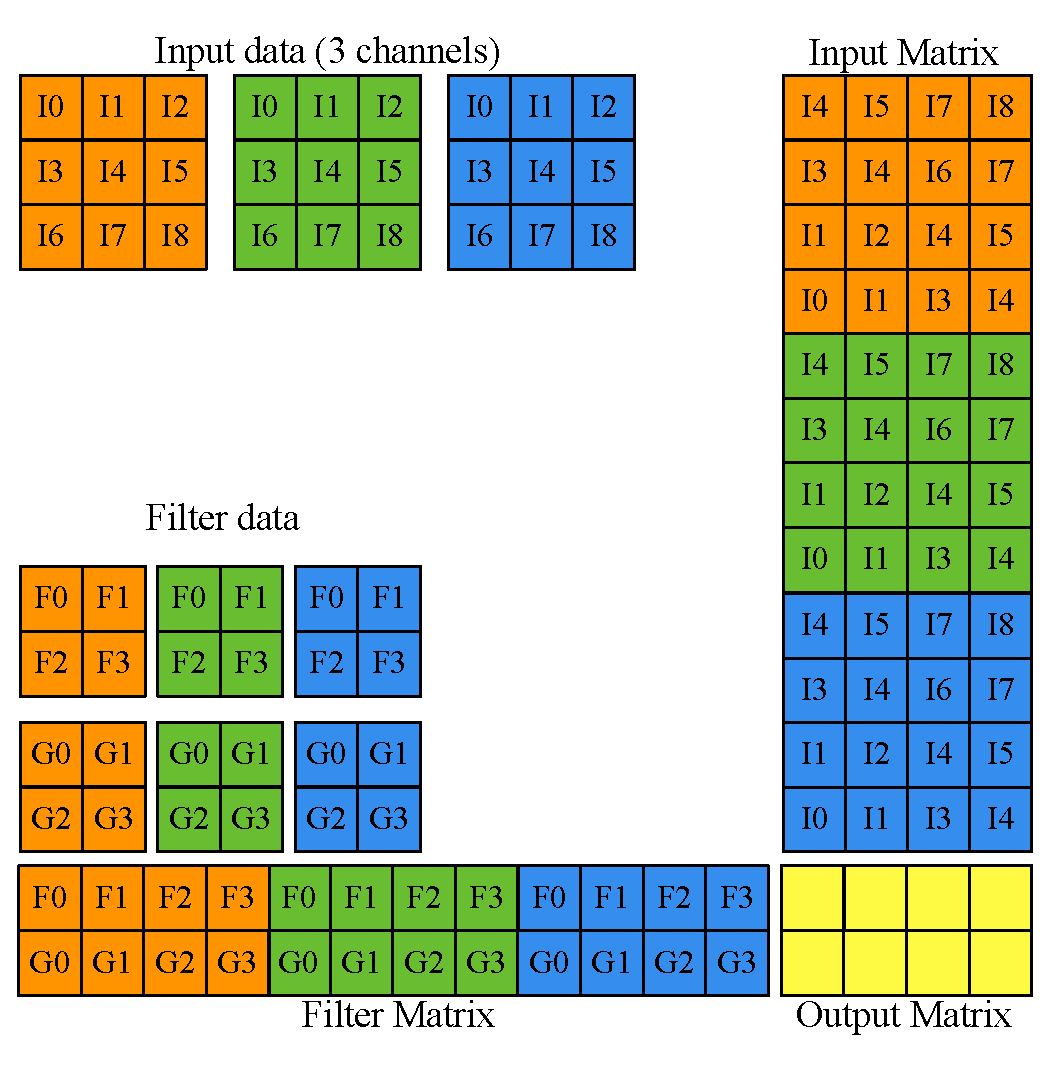
\includegraphics[width=0.85\columnwidth]{./figure/convlowering.eps}
  \caption{An example (reproduced from \cite{ChetlurWVCTCS14}) of converting convolution into matrix multiplications. Here, two filters are applied to a 3-channel input.}
  \label{fig:convlowering}
  \vspace{-3mm}
\end{figure}

Our work targets three representative convolution operations: single-channel, deep-wise and multi-channel 2D convolutions. The
computational kernel of 2D convolution takes as input a 2D single-channel feature map and a channel filter. The filter slides over the
input feature map to perform an element-wise multiplication over the input elements within the filter. Depth-wise convolution takes as
input a 2D feature map and a bank of 2D filters. Each filter is convolved with the corresponding input channel to produce one output
channel. In the multi-channel 2D convolution, all filters are used to convolve with the same input feature map to compute one output
feature map.



Representative algorithms for convolution operations, including GEMM-, FFT- and Winograd-based convolutions, all require to transform 4D
tensors into a transformed matrix where computation can be performed. Doing so can incur high memory overhead. Figure
\ref{fig:convlowering} illustrates the process of GEMM-based convolution, where two filters are applied to a 3-channel input data. All data
are organized as a 4-element tuple, $(batch\_size, channel\_size, height, width)$. The dimension of the filter data in Figure
\ref{fig:convlowering} is $(2, 3, 2, 2)$. The transformed filter matrix has the same number of elements as the filter data. The input data
are of size $(1, 3, 3, 3)$ and have 27 elements in total. However, after transforming the input data into an input matrix, the resulting
matrix would have 48 elements, 44\% of which are redundant. The redundant elements thus lead to additional, redundant memory accesses for
loading and storing the matrix elements. Our work aims to eliminate such redundant elements to reduce the overhead for memory accessing.


\begin{figure}[t!]
\centering
  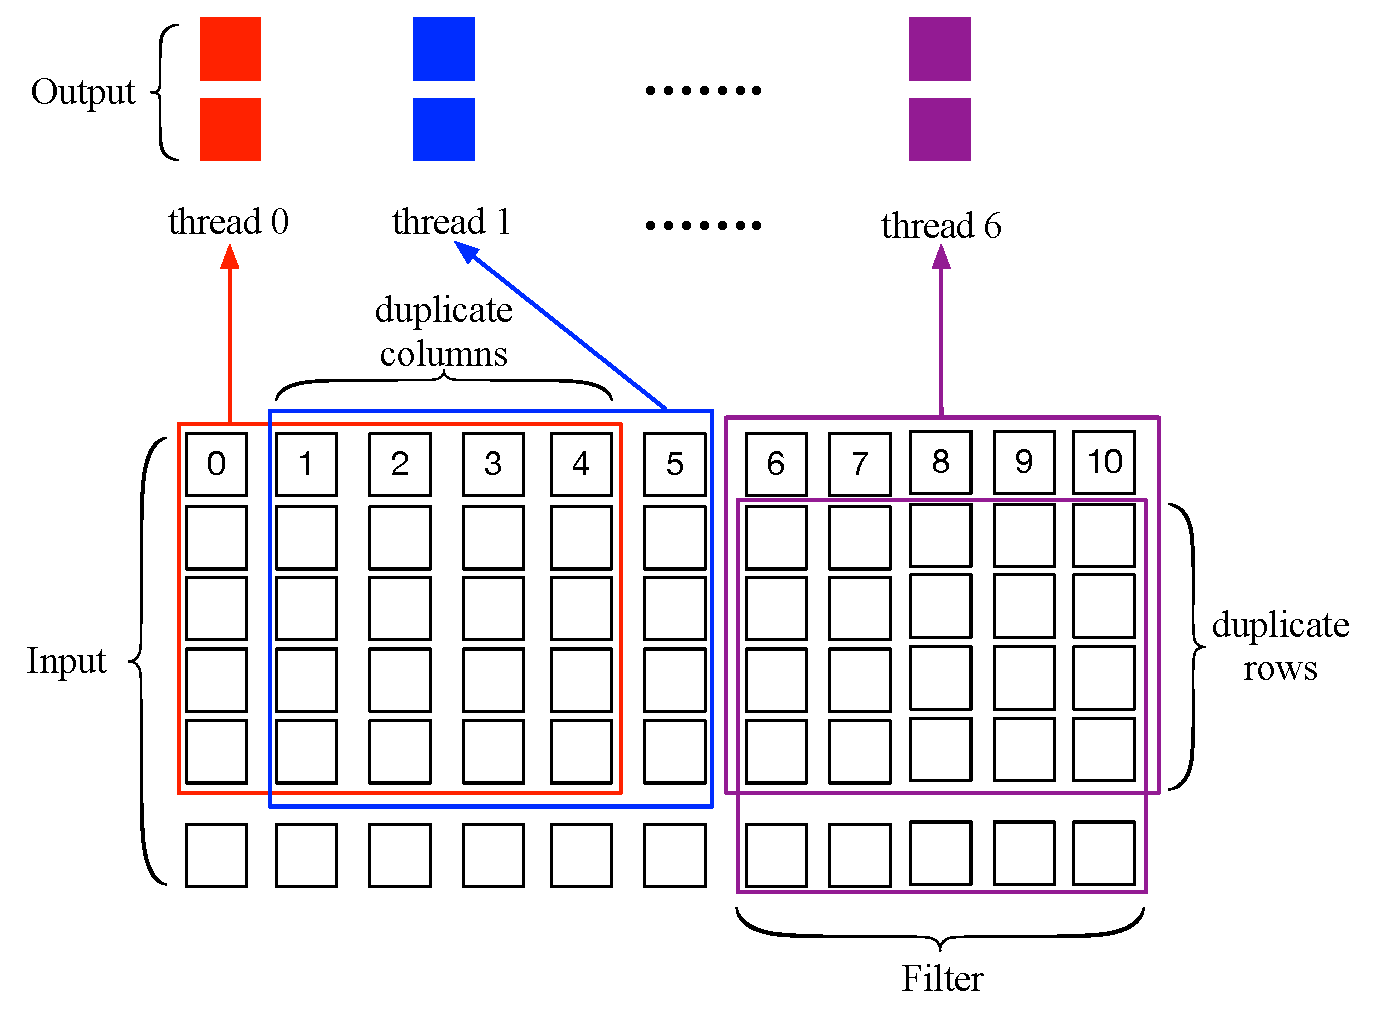
\includegraphics[width=0.9\columnwidth,height=5.5cm]{./figure/twostrategies.eps}
  \caption{Example of performing a 2D convolution using a GPU. Here, the filter size is $5 \times 5$, the input image size is $6 \times 11$
  and the output size is $2 \times 7$.}
  \label{fig:twostrategies}
\end{figure}
